\section{Mass Spring Damper}
\label{sec:massspringdamper}

\subsection{Example Description}
\label{sec:massspringdamper_desc}

The mass spring damper pilot study demonstrates a stabilization technique for co-simulation. The study comprises two mass spring dampers as illustrated in Figure~\ref{fig:msdoverview}. 

\begin{figure}[htbp]
\begin{center}
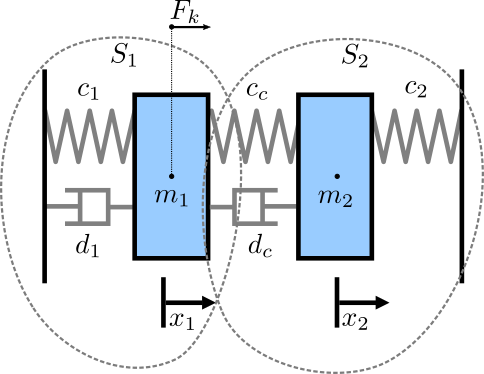
\includegraphics[width=0.5\textwidth]{massSpringDamper/MSDOverview}
\caption{Illustration of two mass spring damper system}
\label{fig:msdoverview}
\end{center}
\end{figure}

There are two simulators included in the study, each representing a mass spring damper system. The first simulator calculates the mass displacement and speed of \emph{m1} for a given force \emph{Fk} acting on mass \emph{m1}. The second simulator calculates force \emph{Fk} given a displacement and speed of mass \emph{m1}.

By coupling these simulators, the evolution of the position of the two masses can be computed by a standalone numerical solver operating directly on the differential equations, to give the expected behaviour illustrated in Figure~\ref{fig:msdexpected}. 


\begin{figure}[htbp]
	\begin{center}
		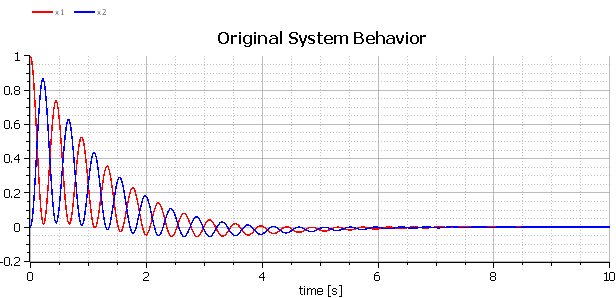
\includegraphics[width=0.7\textwidth]{massSpringDamper/MSDExpected}
		\caption{The expected behaviour of the modelled masses}
		\label{fig:msdexpected}
	\end{center}
\end{figure}

\subsection{Usage}
\label{sec:masspringdamper_usage}

The example is available from the INTO-CPS application menu at \emph{File>Import Example Project} or at \url{https://github.com/into-cps/case-study\_mass\_springer\_damper} in the \emph{master} branch. There are several subfolders for the various elements: \texttt{FMUs} contains the various FMUs of the study; \texttt{Models} -- contains the constituent models defined using the INTO-CPS simulation technologies; \texttt{Multi-models} -- contains two multi-model configurations, for both stable and unstable simulation.

The \texttt{case-study\_mass\_springer\_damper} folder can be opened in the INTO-CPS application to run the various co-simulations as detailed in this document. To run a simulation, expand one of the multi-models and click `Simulate' for an experiment. 

\subsection{Multi-model}
\label{sec:singletank_into_mm}

\subsubsection{Models}
\label{sec:singletank_into_models}

There are several models included in this pilot: a 20-sim model and three OpenModelica models.

\begin{description}
\item[MassSpringDamper.emx] The 20-sim model of the two spring damper example, shown in Figure~\ref{fig:msd20sim}, comprises a sub-component for each spring damper. Each sub-component describes the dynamics of the spring damper, and the two sub-components are connected. \emph{MassSpringDamper1} calculates displacement and velocity of a mass for a given force acting on it. \emph{MassSpringDamper2} calculates the resulting force from a given a mass displacement and velocity.

\begin{figure}[htbp]
	\begin{center}
		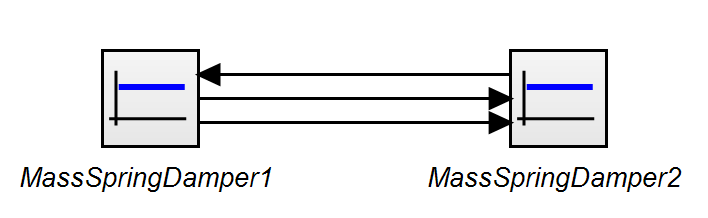
\includegraphics[width=0.35\textwidth]{massSpringDamper/massSpringDamper20sim}
		\caption{20-Sim model of Mass Spring Damper System}
		\label{fig:msd20sim}
	\end{center}
\end{figure}


\item[MassSpringDamper1.mo] \emph{MassSpringDamper1.mo} describes the same dynamics expressed in \emph{MassSpringDamper1} in the 20-sim model \emph{MassSpringDamper.emx}.

\item[MassSpringDamper2.mo] \emph{MassSpringDamper2.mo} describes the same dynamics expressed in \emph{MassSpringDamper2} in the 20-sim model \emph{MassSpringDamper.emx}.
 
\item[MassSpringDampersScenario.mo] \emph{MassSpringDampersScenario.mo} links MassSpringDamper1.mo and MassSpringDamper2.mo and defines parameters for simulation.

\end{description}

\subsubsection{Configuration}
\label{sec:masspringdamper_conf}
A single multi-model is defined:
\begin{description}
\item[mm] The multi-model \texttt{mm} uses the \emph{20-sim/MassSpringDamper1.fmu} and \\ \emph{20-sim/MassSpringDamper2.fmu} FMUs.

There are several design parameters defined the multi-model configuration.
\end{description}

\subsection{Co-simulation}
\label{sec:masspringdamper_co}

Two co-simulation variations are defined for the multi-model. Both simulation configurations have identical parameters, including a runtime of 10 seconds and use a fixed step size of 0.001 seconds. The only difference between the two configurations is the application of COE stabilisation (successive substitution).

\begin{description}
	\item[Unstable] This co-simulation configuration does not enable stabilisation. Co-simulating this multi-model configuration produces the output plotted in Figure~\ref{fig:msd_unstable}, which shows two trajectories increasing indefinitely. This differs greatly from the expected output illustrated in Figure~\ref{fig:msdexpected} where the two trajectories tend to 0 over time.

\begin{figure}[htbp]
	\begin{center}
		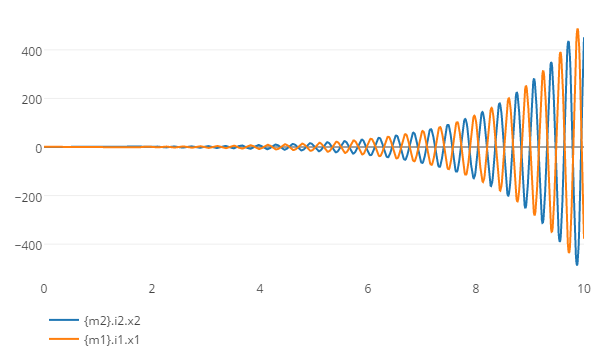
\includegraphics[width=0.7\textwidth]{massSpringDamper/massSpringDamperUnstable}
		\caption{Co-simulation output of unstable configuration}
		\label{fig:msd_unstable}
	\end{center}
\end{figure}

	\item[Stable] This co-simulation configuration does enable stabilisation. Co-simulating this multi-model configuration produces the output plotted in Figure~\ref{fig:msd_stable}, which shows the expected behaviour as illustrated in Figure~\ref{fig:msdexpected}.
	
\begin{figure}[htbp]
	\begin{center}
		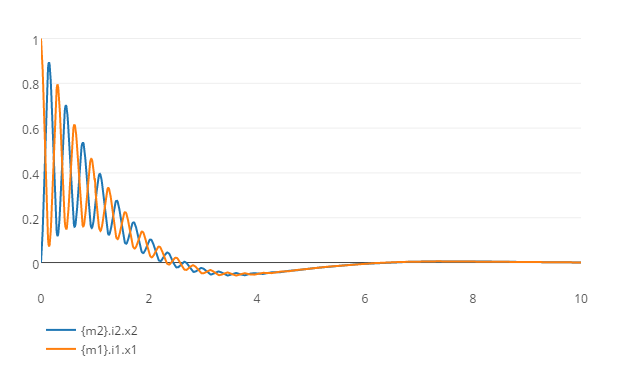
\includegraphics[width=0.7\textwidth]{massSpringDamper/massSpringDamperStable}
		\caption{Co-simulation output of stable configuration}
		\label{fig:msd_stable}
	\end{center}
\end{figure}	
\end{description}
